
\documentclass[11pt,a4paper]{article}
\usepackage[hyperref]{acl2020}
\usepackage{times}
\usepackage{latexsym}
\renewcommand{\UrlFont}{\ttfamily\small}

% This is not strictly necessary, and may be commented out,
% but it will improve the layout of the manuscript,
% and will typically save some space.
\usepackage{microtype}
\usepackage{graphicx}

\aclfinalcopy % Uncomment this line for the final submission
%\def\aclpaperid{***} %  Enter the acl Paper ID here

%\setlength\titlebox{5cm}
% You can expand the titlebox if you need extra space
% to show all the authors. Please do not make the titlebox
% smaller than 5cm (the original size); we will check this
% in the camera-ready version and ask you to change it back.

\newcommand\BibTeX{B\textsc{ib}\TeX}

\title{COMP90042 Natural Language Processing\\
Project Report\\
2020 Semester 1}

\author{Rongbing Shan, 945388, rashan@student.unimelb.edu.au}

\date{2020-05-12}

\begin{document}
\maketitle
\begin{abstract}
The growing attention on climate change has caused more misinformation on the subject found on different media. In this project for COMP90042, a misinformation detection system is developed to automatically identify misinforamtion on climate change topics. In this report of the project, the implementation on the detection system is discussed, using one class classifier and binary classifers. The peformances of each apporach are also adressed and discussed.
\end{abstract}

\section{Introduction}

The global fucus on climate change has been continously growing for the last few years, and people are more and more concerned about the environment problem. It is generally believed that human activities have caused big problems on climate environment. However, as the focus on problem grows, there comes many rumours on this topic [1], which are hard to distinguish merely by human.
In this project of COMP90042, we are required to develop a misinformation detection system on rumours about climate change using natural language processing techniques. A dataset of only positive labels(misinformation) is provided for this project.
Commonly, for an automatic fact check problem like in this project, there are two possible ways for the detection: \textbf{Linguistic Approach} and \textbf{Network Approach}. For Linguistic Approach, the deceptive content should be extracted based on language patterns. The misinforamtion would have some similiar language patterns such as fear mongering. While for Network Approach, the metadata for the information can be taken into consideration, such as the source or author for the information. An information from a unreliable source is likely to be a misinformation. In this report, we will consider only the \textbf{Linguistic Approach} as described above. 
The system is developed using two different approaches, One Class SVM and Random Forest.
Also, a colab competition is run together with this project, and the performance on the competetion final result will also be discussed in this report.

\section{Background}
In this section, background will be introduced.

\subsection{Dataset}
There are two training datasets used in the project: one is provided with only positive labels(misinformation), the other is collected from EventRegistry with negtive lables. Besides, there is a dev dataset for hyperparameter tunning and also for the major discussion in this report. At last there is also a test dataset to compete over on colab.
\begin{table}[h!]
  \begin{center}
    \caption{Dataset summary}
    \label{tab:table1}
    \begin{tabular}{l|c|r}
      \textbf{Dataset} & \textbf{NumOfDocs} & \textbf{Labels}\\
       $filename$ & $count$ & $1/0$ \\
      \hline
      train.json & 1168 & 1168/0\\
      negative-train.json & 1100 & 0/1100\\
      dev.json & 100 & 50/50\\
      test-unlabelled.json & 1410 & unknown\\
    \end{tabular}
  \end{center}
\end{table}

\subsection{Automated Fact Check}
This project can be categoried to the problem of automated fact check. By automated fact check, we mean the development of a automated system or tool to help human identifying and verifying the factual status of statements. According to Hassan [2], an automated fact checking sytem is \textbf{Fully Automated},\textbf{Accurate},\textbf{Instant} and \textbf{Accountable}. Fully automated means the system can check facts without human intervention, Instant means it immediately gets conclusion and return the results. And Accurate means it should be at least same accurate as human checker or more accurate. Accountable states that the system should be transparent on its sources and analysis process, so that it can be verified, repeated and improved.

\section{Methodology}

In this section, methodologies in the project will be introduced, including the feature engineering on datasets, training models used.
\subsection{Feature Engineering}
there are two possible ways for the detection: \textbf{Linguistic Approach} and \textbf{Network Approach}. And the main difference on the two approaches lies in feature engineering: Network approach would reverse engineering the information and acquire its source metadata as a feature for training. However, this is not permitted in this project. Hence, we will be focusing on only Linguistic Apporach.\\
For the linguistic approach, we are supposed to identify facts based on only the text information. Most misinformation creators would use certain language strategies to avoid being caught, or to increate its credibility to the audiance, such as fear mongering or denying on the science. Therefore, features are most important part in such an approach, how the features can capture the language patterns for misinformation will directly impact the accuracy of the whole misinformation detection system.\\
According to [3], features used in linguistic approach can be generally divided into three categories: \textbf{Data Representation},\textbf{Deep Syntax} and \textbf{Semantic Analysis}.\\ Here in my implementation, I would divide the features to similar categories: \textbf{Simple Word Features}, \textbf{Stylistic Features} and \textbf{Emotional Features}.



\paragraph{Simple Word Features:}
The simpliest eay for representing text would be bag of words apporach, which regard the words in a text as seperated, equally important tokens. Although simple, the representation method can give much information on the text itself, as in our problem if a text contains no word related to climates or environment, it is very much likely a negative case(not climate change misinforamtion). In this project, both word count and TF-IDF representation are used in simple word features. However, this method also leads to a big shortcomming, it can only represents simple word mentions in the information, but unable to capture syntax or styles that misinformation can used. An proper information on climate change and misinformation may use very similiar tokens, but the diffferent language syntax and structure leads to totoally different meaning.

\paragraph{Stylistic Features:}
The Stylistic aims to capture the grammatical element, syntax and text styles in the data. In my implementaiton, the Part of Speach(POS) tagger in Python Natural Language Toolkit(NLTK) is used to test differences in syntax. The count for each tag is kept as features. Also, the number of links, number of stop words, average tokens per sentence will also be captured to address the complicity of the text information. It is believed that such information will generally give an instruction on whether the information is true or not, since misinformation creators may choose to repeat the same words serval times to credit the reader.

\paragraph{Emotional Features:}
The emotional features are based on some selected word categories that could address the emotion or psychology of the information creator. we would address causual words, contrast words and negation words in the implementation, since for a misinforamtioin creator, it is likely he will use more such words to explain its theory and convince the audiance.
Also, a sentiment analysis score is addressed in the implementation since the author would likely to show stronger emotions when writing a fake article on climate change. TextBlob in python is used to capture such sentiment scores, as well as a score for subjectivity, since misinformation tends to be not very objective.
\begin{table*}[h]
  \begin{center}
    \caption{Features}
    \label{tab:table2}
    \begin{tabular}{l|c|r}
      \textbf{Category} & \textbf{Name} & \textbf{Description}\\
      \hline
SimpleWord & BOW* & word count\\
SimpleWord & TF-IDF* & term frequency, inverse document frequency\\
Stylistic & POS & 35 POS tag counts \\
Stylistic & url count & count of URLs in the document\\
Stylistic & stopword count & count of stopwords in the document\\
Stylistic & avg word per sentence & average number of words per sentence\\
Stylistic & stopword pct & percent of stopwords in a document\\
Stylistic & punctuation pct & percent of punctuations in a document\\
Stylistic & lexical diversity & percent distinct words in a document\\
Emotional & doc sentiment & TextBlob sentiment score for a document\\
Emotional & doc objectivity & TextBlob objectivity score for a document\\
Emotional & pos sent count & count of postive sentence in a document\\
Emotional & neg sent count & count of negative sentence in a document\\
Emotional & max sent sentiment & maximum score of sentence sentiment in a document\\
Emotional & min sent sentiment & minimum score of sentence sentiment in a document\\
Emotional & causual word & count of causual words\\
Emotional & contrast word & count of contrast words\\
Emotional & negation word & count of negation words\\
    \end{tabular}
    \texttt{ note: * either one of BOW or TF-IDF is used}
  \end{center}
\end{table*}

\subsection{Models}
Three models are used in the project to create the dection system, one for one class classification and one for binary class classification:\textbf{One Class SVM} and \textbf{Random Forest}."train.json" and "negative.json" dataset will be used in training process. Hyper parameter tunning will be conducted on dev.json dataset. And colab competition is run on 'test-unlabelled.json'.

\section{Evaluation and Analysis}
In this section, the result of different models will be discussed. Errors will be analysed and performance will be compared.
\subsection{Baseline}
In this project, a random baseline is provided. No other models will be trained as baseline model.
\begin{table}[h!]
  \begin{center}
    \caption{Baseline}
    \label{tab:table1}
    \begin{tabular}{c c c}
      \textbf{F1} & \textbf{P} & \textbf{R}\\
      \hline
      0.54 & 0.51 & 0.56\\
    \end{tabular}
  \end{center}
\end{table}

\subsection{One class SVM}
One Class SVM is trained over 4 sets of different features to see the impact of feature engineering on performance.
\begin{table}[h!]
  \begin{center}
    \caption{One Class SVM Performance}
    \label{tab:table1}
    \begin{tabular}{c c c c}
      \textbf{Feature} & \textbf{F1} & \textbf{P} & \textbf{R}\\
      \hline
      BOW & 0.74 & 0.68 & 0.82\\
      BOW + all & 0.70 & 0.625 & 0.80\\
      TF-IDF & 0.71 & 0.60 & 0.84\\
      TF-IDF + all & 0.68 & 0.59 & 0.8\\
    \end{tabular}
  \end{center}
\end{table}

\paragraph{Analysis:}
The model overruns baseline in both precision and recall of postive class, and it performes well in finding the postive class, which generates a high recall above 0.8. However, the precision is relatively lower than expected, indicating the model classifies many negative document as misinformation.
With further look into details on the predictions, we find the classifier identifies many negative cases as postive, which generating the result of high recall and low precision.
Also, it is supurised to see that with additional stylistic features and emotional features, the performance of the classifier drops. That's probably because the svm model do not priorities the features and there are over 20000 tokens while only 30+ other features, the importance of additional features are lowered.

\subsection{Random Forest}
Random Forest Classifier is also trained over 4 sets of different features. However, compared to OCSVM, negative training set are included.
\begin{table}[h!]
  \begin{center}
    \caption{Random Forest}
    \label{tab:table1}
    \begin{tabular}{c c c c}
      \textbf{Feature} & \textbf{F1} & \textbf{P} & \textbf{R}\\
      \hline
      BOW & 0.72 & 0.61 & 0.88\\
      BOW + all & 0.743 & 0.61 & 0.94\\
      TF-IDF & 0.72 & 0.61 & 0.88\\
      TF-IDF + all & 0.73 & 0.62 & 0.90\\
    \end{tabular}
  \end{center}
\end{table}

\paragraph{Analysis:}
This model also overruns baseline in all aspects.Random Forest Classifier does even better in finding out all the positive labels, hence a better recall close to 1. But the precision is still relatively lower than expected.
In Random Forest, stylistic and emotional features gives a clearly larger impact on the improvement of performance, which is due to RF can prioritise features.
This model still can be improved in its precision, which I think can be improved by introducing more training datasets, on both positive and negative class. Also, more features can be added, details will be discussed more in following sections.

\subsection{Comparison Between Models}
By comparing the best perfomrance model from One Class SVM and Random Forest, Random Forest has a similiar but slightly better performance than One Class SVM. By treating the problem as binary classfication instead of novelty detection, the performance is improved.That's probably because with introducing on the negative dataset, the syntax and property of the text are better addressed. Also, random forest can prioritize the features, so compard with svm, it can better utilize the stylistic and emotional features introduced. From the result on RF, this point is also proved.

\begin{figure}[h!]
  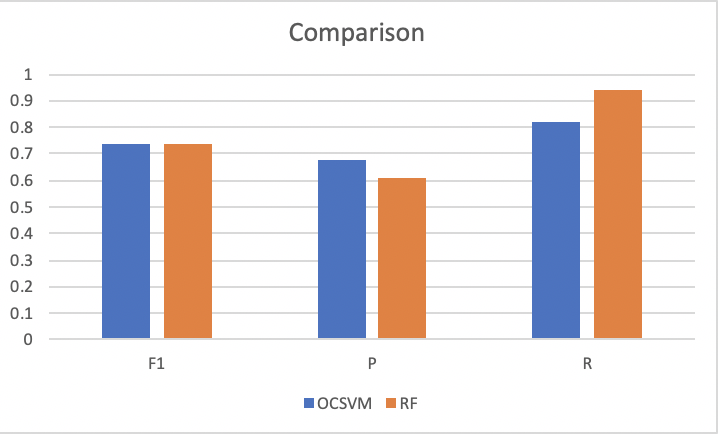
\includegraphics[width=\linewidth]{compare.png}
  \caption{Comparison of two models}
  \label{fig:figure1}
\end{figure}

\section{Future Improvements}
There are some future development directions learned from analysing result of the project.
\paragraph{feature engineering:}
Currently a full bag of words is used as features, but many of the tokens are not related to the climate change topic. In future developments, some tokens not related to the topic of study can be removed and only tokens related should be kept. Also there can be more emotional features, Linguistic Inquiry and Word Count (LIWC) can be used to address tokens in more disciplines like 'analytic', 'differ', 'risk', etc. Besides, Probability Context Free Grammars (PCFG) can also be addressed to better understand the syntax of text.
\paragraph{data collection:}
In the project, only thousand training data are used, which is a bit small. More positive data can be collected for training purpose.
\paragraph{models:}
More models can be tried like autoencoders and neural networks for claissification.

\section{Colab Competition}
The result of my implementation on colab comes with following result.
\begin{table}[h!]
  \begin{center}
    \caption{Colab Rank}
    \label{tab:table5}
    \begin{tabular}{l|c|r}
      \textbf{F1} & \textbf{Precision} & \textbf{Recall}\\
      \hline
   0.52(209) & 0.36(215) & 0.92(9)\\
    \end{tabular}
  \end{center}
\end{table}
The result is the best ongoing model submitted. However, this model is trained with only TF-IDF word representation with no other features included using one class svm. From above discussion, we can see that Random Forest models gives much better performance on development dataset, but on test dataset, its performance drops. This can be caused by that the features are not good enough to capture syntax and structure and also the dataset used for training is a bit small in size. These two reasons caused the system to have a lower generality.

\section{Conclusion}
In the project, random forest classifer gives the best result on development dataset but a lower performance on test dataset. Although the general improvement compared to random baseline is good, there is still much improvement space, especially of performance on test datset. It is assumed that the features are not good enough to capture the syntax. Also, the training dataset is a bit small, more postive label dataset should be collected for training for a better performance.
Also, it is learned that feature engineering plays a very important role when we are using Linguistic approaches. Whether the features are capable to capture the deep syntax and structure of the text is highly related to the accuracy of the system. Besides, dataset used in training may also highly impact the results on the colab competition board.

\section*{Reference}
[1] Van der Linden, Sander, et al. "Inoculating the public against misinformation about climate change." Global Challenges 1.2 (2017): 1600008. \\\relax
[2] Hassan, Naeemul, et al. "The quest to automate fact-checking." Proceedings of the 2015 Computation+ Journalism Symposium. 2015.\\\relax
[3] Conroy, Niall J., Victoria L. Rubin, and Yimin Chen. "Automatic deception detection: Methods for finding fake news." Proceedings of the Association for Information Science and Technology 52.1 (2015): 1-4.\\\relax

\end{document}
